\section{Modern concept of digital image}

A digital image is a numerical representation of a visual scene,
captured through various imaging devices and stored in a computer.
From a mathematical perspective, a digital image can be represented
as a function $f(x,y)$ that maps spatial coordinates $(x,y)$ to
intensity values. In the discrete domain, this function is sampled at
regular intervals, creating a matrix of values known as pixels
(picture elements).

\subsection{Types of digital images}

\subsubsection{Grayscale images}
Grayscale images are the simplest form of digital images, where each
pixel represents a single intensity value. Mathematically, a
grayscale image can be represented as a 2D matrix $I$ of size $M
\times N$, where each element $I(i,j)$ represents the intensity at
position $(i,j)$. The intensity values typically range from 0 (black)
to 255 (white) in 8-bit images, or from 0 to 65535 in 16-bit images.

\subsubsection{Color images}
Color images extend the grayscale concept by representing each pixel
with multiple channels, typically Red, Green, and Blue (RGB). A color
image can be represented as a 3D matrix $I$ of size $M \times N
\times 3$, where $I(i,j,k)$ represents the intensity of the $k$-th
color channel at position $(i,j)$. Other color spaces like HSV (Hue,
Saturation, Value) or CMYK (Cyan, Magenta, Yellow, Key) are also
commonly used in different applications.

\subsubsection{Multispectral images}
Multispectral images capture information across multiple wavelength
bands beyond the visible spectrum. These images can be represented as
a 3D matrix $I$ of size $M \times N \times B$, where $B$ is the
number of spectral bands. Each band $I(i,j,b)$ represents the
intensity at position $(i,j)$ for the $b$-th spectral band. This
representation is particularly useful in medical imaging, remote
sensing, and scientific applications.

\subsubsection{3D images and volumetric data}
Three-dimensional images extend the concept of pixels to voxels
(volume elements). A 3D image can be represented as a 3D matrix $V$
of size $M \times N \times D$, where $D$ represents the depth
dimension. Each voxel $V(i,j,k)$ represents the intensity at position
$(i,j,k)$ in the 3D space. This representation is fundamental in
medical imaging (CT, MRI), scientific visualization, and computer graphics.

\subsection{Mathematical representations}

The mathematical foundation of digital images relies on several key concepts:

\begin{itemize}
  \item \textbf{Sampling}: The process of converting a continuous
    image into a discrete representation. According to the
    Nyquist-Shannon sampling theorem, the sampling frequency must be
    at least twice the highest frequency present in the image to avoid aliasing.

  \item \textbf{Quantization}: The process of converting continuous
    intensity values into discrete levels. The number of quantization
    levels determines the image's bit depth and affects its quality
    and storage requirements.

  \item \textbf{Resolution}: The number of pixels per unit length in
    an image, typically measured in pixels per inch (PPI) or dots per
    inch (DPI).

  \item \textbf{Dynamic range}: The ratio between the maximum and
    minimum measurable light intensities in an image, often expressed
    in decibels (dB).
\end{itemize}

The mathematical representation of a digital image can be expressed as:

\begin{equation}
  I(x,y) = \sum_{i=0}^{M-1} \sum_{j=0}^{N-1} f(i,j) \cdot \delta(x-i, y-j)
\end{equation}

where $I(x,y)$ is the digital image, $f(i,j)$ represents the
intensity values, and $\delta(x-i, y-j)$ is the Kronecker delta function.

For color images, the representation extends to:

\begin{equation}
  I(x,y) =
  \begin{bmatrix}
    I_R(x,y) \\
    I_G(x,y) \\
    I_B(x,y)
  \end{bmatrix}
\end{equation}

where $I_R$, $I_G$, and $I_B$ represent the red, green, and blue
channels respectively.

\begin{figure}[htbp]
  \centering
  \begin{tikzpicture}[
      node distance=2cm,
      block/.style={draw, rectangle, minimum width=2cm, minimum
      height=1.5cm, align=center},
      arrow/.style={->, >=stealth, thick},
      label/.style={font=\small}
    ]

    % Main image concept
    \node[block] (main) {Digital Image};
    \node[block, below left=of main] (grayscale) {Grayscale};
    \node[block, below=of main] (color) {Color};
    \node[block, below right=2.5cm and 1cm of main] (multispectral)
    {Multispectral};
    \node[block, below right=1cm and 3.5cm of main] (volumetric)
    {3D/Volumetric};

    % Mathematical representations
    \node[block, below=of grayscale] (gray_math) {2D Matrix\\$M \times N$};
    \node[block, below=of color] (color_math) {3D Matrix\\$M \times N
    \times 3$};
    \node[block, below=of multispectral] (multi_math) {3D Matrix\\$M
    \times N \times B$};
    \node[block, below=of volumetric] (vol_math) {3D Matrix\\$M
    \times N \times D$};

    % Sampling and quantization
    \node[block, left=of main] (sampling) {Sampling};
    \node[block, right=of main] (quantization) {Quantization};

    % Connect main concept to types
    \draw[arrow] (main) -- (grayscale);
    \draw[arrow] (main) -- (color);
    \draw[arrow] (main) -- (multispectral);
    \draw[arrow] (main) -- (volumetric);

    % Connect types to mathematical representations
    \draw[arrow] (grayscale) -- (gray_math);
    \draw[arrow] (color) -- (color_math);
    \draw[arrow] (multispectral) -- (multi_math);
    \draw[arrow] (volumetric) -- (vol_math);

    % Connect sampling and quantization
    \draw[arrow] (sampling) -- (main);
    \draw[arrow] (quantization) -- (main);

    % Add labels
    \node[label, above=0.5cm of main] {Digital Image Concepts};
    \node[label, above=0.5cm of sampling] {Processes};
    \node[label, above=0.5cm of quantization] {Processes};

    % Add example images placeholders
    \node[draw, rectangle, minimum width=2cm, minimum height=1.5cm,
    below=0.5cm of gray_math] (gray_ex)
    {
\includegraphics[width=2cm]{Cap2/Figures/gray_example.jpg}};
    \node[draw, rectangle, minimum width=2cm, minimum height=1.5cm,
    below=0.5cm of color_math] (color_ex)
    {
\includegraphics[width=2cm]{Cap2/Figures/color_example.png}};
    \node[draw, rectangle, minimum width=2cm, minimum height=1.5cm,
    below=0.5cm of multi_math] (multi_ex)
    {
\includegraphics[width=2cm]{Cap2/Figures/multispectral_example.png}};
    \node[draw, rectangle, minimum width=2cm, minimum height=1.5cm,
    below=0.5cm of vol_math] (vol_ex)
    {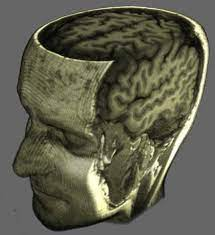
\includegraphics[width=2cm]{Cap2/Figures/volumetric_example.jpg}};

    % Connect mathematical representations to examples
    \draw[arrow] (gray_math) -- (gray_ex);
    \draw[arrow] (color_math) -- (color_ex);
    \draw[arrow] (multi_math) -- (multi_ex);
    \draw[arrow] (vol_math) -- (vol_ex);

  \end{tikzpicture}
  \caption{Overview of digital image concepts and their mathematical
    representations. The figure shows the main types of digital images
    (grayscale, color, multispectral, and volumetric), their
    mathematical representations, and the fundamental processes of
    sampling and quantization. Example images are included to
  illustrate each type.}
  \label{fig:image_concepts}
\end{figure}